\section*{Übung 4}
\subsection*{Aufgabe 1}
\subsubsection*{Lösungsidee}
Für das Umwandeln in andere Basen wird eine allgemeine Formel verwendet. Dazu wird ein String verwendet in dem alle erlaubten Zeichen sind, gleichzeitig wird die Position des Zeichens im String als Wertigkeit des Zeichens in der Basis 10 verwendet.

\lstinputlisting[language=Pascal] {../base2to36.pas}
\begin{figure}[H]
	\centering
	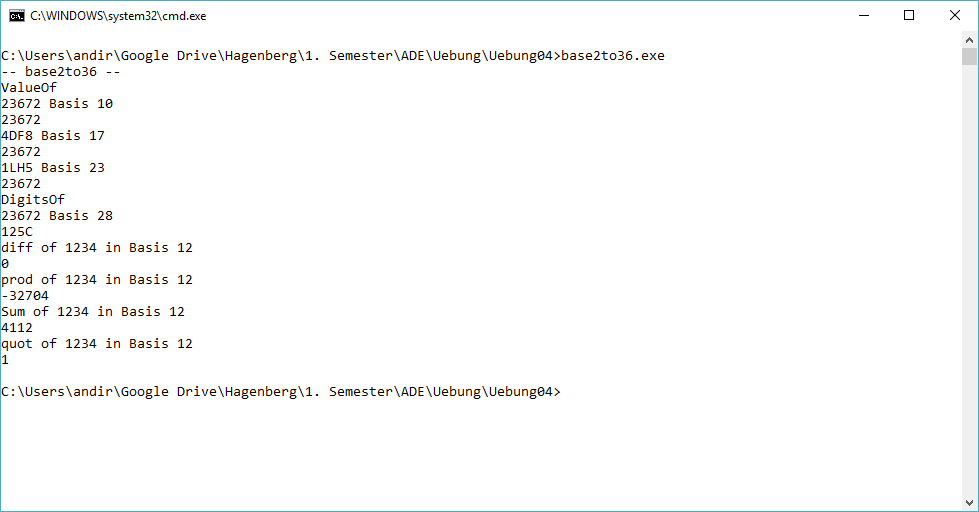
\includegraphics[scale=0.75]{./pictures/base2to36.png}
	\caption{Testfälle Basis 2 bis 36}
	\label{fig: Spannweiten Berechnung}
\end{figure}

\section*{Testfälle}
Zum Testen werden verschiedene Basen verwendet, dabei soll immer dieselbe Zahl ausgegeben werden.
Anschließend wird noch ein Zahl in der 10 Basis in der 28er Basis ausgegeben. Zum Schluss werden Diff, Sum, Prod und quot ausgegeben (mit 1234 in Basis 12), wobei bei Prod eine negative Zahl ausgegeben wird weil der Bereich überschritten wird. Dasselbe kann auch bei Sum passieren wenn zu hohe Zahlen verwendet werden.

\newpage

\subsection*{Aufgabe 2}
\subsubsection*{Lösungsidee}
Beim Balkendiagramm redone wird ein String verwendet an dem immer die jeweilige Zeile für einen Politiker angehängt und anschließend ausgegeben wird.

\lstinputlisting[language=Pascal] {../balkendiagramm_redone.pas}
\begin{figure}[H]
	\centering
	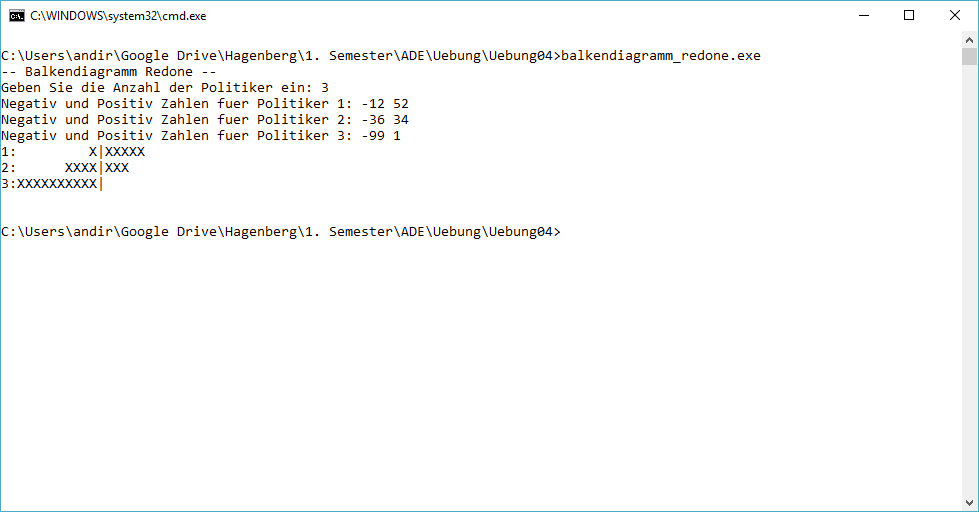
\includegraphics[scale=0.75]{./pictures/balkendiagramm_redone.png}
	\caption{Testfälle Balkendiagramm}
	\label{fig: Sortieralgorithmus}
\end{figure}

\section*{Testfälle}
Es werden drei Politiker eingegeben mit unterschiedlichen Zahlen.

\newpage

\subsection*{Aufgabe 3}
\subsubsection*{Lösungsidee}
Zum finden der fehlenden Zahl wird eine Folge von Zahlen aufsummiert und dann von einer Check Summe abgezogen. Der Rest ist das fehlende Element.

\lstinputlisting[language=Pascal] {../missingelement.pas}
\begin{figure}[H]
	\centering
	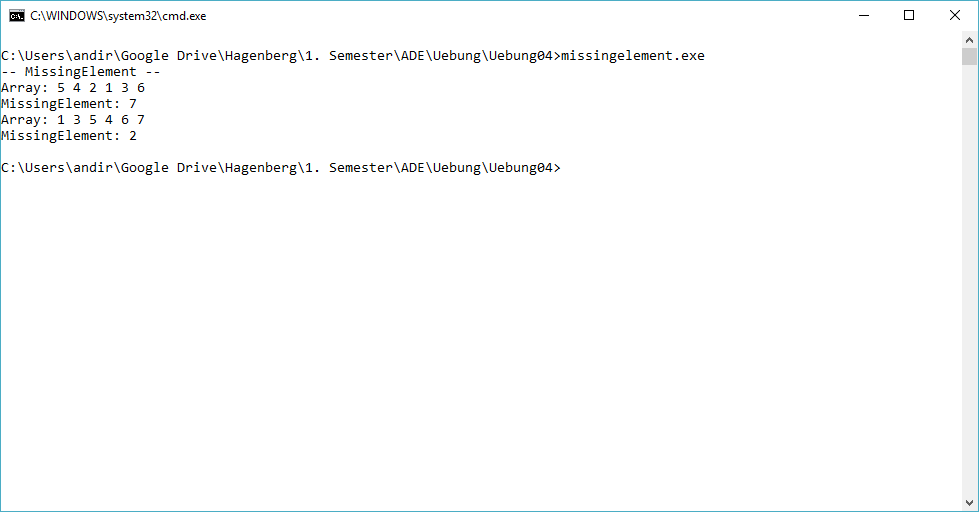
\includegraphics[scale=0.75]{./pictures/missingelement.png}
	\caption{Testfall missingelement}
	\label{fig: label}
\end{figure}

\section*{Testfall}
Ein Array mit einer Test Größe von 7 wird mit Zahlen in beliebiger Reihenfolge gefüllt und das fehlende Element wird ausgegeben. Dasselbe wird mit einem zweiten Array, mit einem anderen fehlenden Element, gemacht.

\newpage